% 五号字体,开明式标点处理,不设置默认字体
\documentclass[UTF8,12pt,punct=kaiming,fontset=none]{ctexart}
\usepackage{fontspec}  % 字体
\usepackage{subcaption}  % 节标题
% 品红色链接和注释
% \usepackage[colorlinks=true, linkcolor=magenta, citecolor=magenta, urlcolor=magenta]{hyperref}
% 黑色链接和注释
\usepackage[colorlinks=true,linkcolor=black,citecolor=black,urlcolor=black]{hyperref}
\usepackage{geometry}  % 页面布局
\usepackage{fancyhdr}  % 页眉页脚
\usepackage{titlesec}  % 标题
\usepackage{caption}  % 图表标题
\usepackage{floatrow}  % 图表排版
\usepackage{graphicx}  % 图片路径
% 表格(可选)
\usepackage{multirow}
\usepackage{boldline}
% 电路图(可选)
\usepackage{tikz}
\usepackage[european,nooldvoltagedirection]{circuitikz}

% 图片路径
\graphicspath{{figures/}}

% 字体
\setCJKmainfont{Source Han Serif SC}
\setCJKsansfont{Source Han Sans SC}
\setmainfont{CMU Serif}

% 布局
\geometry{a4paper,left=2cm,right=2cm,top=2.5cm,bottom=2.5cm}
\setlength{\headheight}{25pt}

% 图表标题
\DeclareCaptionFont{captionfont}{\small}
\captionsetup{font=captionfont}
\floatsetup{style=plaintop}

% 页眉页脚
\pagenumbering{arabic}
\pagestyle{fancy}
\fancyhead[L]{· \hspace{0.1cm} \thepage \hspace{0.1cm} ·}
\fancyhead[C]{红 \hspace{0.08cm} 石 \hspace{0.08cm} 数 \hspace{0.08cm} 电 \hspace{0.08cm} 评 \hspace{0.08cm} 论\\\scriptsize{Review of Redstonic Digital Circuit}}
\fancyhead[R]{第1期\\\scriptsize{2022年1月}}
\fancyhead[C]{红~石~数~电~评~论\\\scriptsize{Review of Redstonic Digital Circuit}}
\fancyhead[R]{2022年1月(第1期)}
\fancyfoot[L,C,R]{}

% 首页页码
\setcounter{page}{1}

% 标题
\title{\vspace{-1.5cm}潜影盒倒序装填器\vspace{-0.5cm}}
\author{@redberd\thanks{作者联系方式~\url{https://space.bilibili.com/14122148}}~\textsuperscript{,}\thanks{TIS Trinity Union服务器}}
\date{}

% 参考文献标注
\newcommand*{\upcite}[1]{
    \textsuperscript{\cite{#1}}
}

\begin{document}
\maketitle
\thispagestyle{fancy} % 首页页眉页脚
\vspace{-0.7cm}

% 节标题格式
\titleformat{\section}[hang]{\large\sffamily\bfseries}{\textmd{\thesection}}{0.5cm}{}
\titlespacing{\section}{0cm}{0.5ex}{0.2ex}
\titleformat{\subsection}[hang]{\normalsize\sffamily}{\textmd{\thesubsection}}{0.5cm}{}
\titlespacing{\subsection}{0cm}{0.5ex}{0.2ex}
\setcounter{section}{0}

潜影盒倒序装填器,是一种将物品流自动装进潜影盒,同时保存物品的顺序信息的装置。利用该装置,可以做出可重复读取、大容量、高密度的潜影盒ROM\upcite{ref1},有良好的发展前景。目前,倒序装填技术在编码红石音乐领域有重要的应用\upcite{ref2}。

普通的潜影盒装填器,或叫做“打包机”,只是单纯地把物品装进潜影盒中,而物品流的顺序信息往往会丢失。这是因为,漏斗将物品装入容器时,会优先把物品填入容器中靠前的格子里。若在物品流中,存在两个相同的可堆叠物品,但不相邻,那么这两个物品就会堆叠在同一个格子里。这时,就无法根据潜影盒的内容判断,这两个物品原先是否相邻,即物品流的顺序信息丢失。

本文提出的潜影盒倒序装填器,运用了倒序装填的方法\upcite{ref3},从而能保存物品流的顺序信息。倒序装填,就是向容器的格子中从后往前依次填入物品,即从潜影盒的第27格开始,依次填入物品,一直填到第1格。这样就能避免相同且不相邻的物品堆叠在一起了,从而保存了物品流的顺序信息。

\begin{figure}[h]
    \centering
    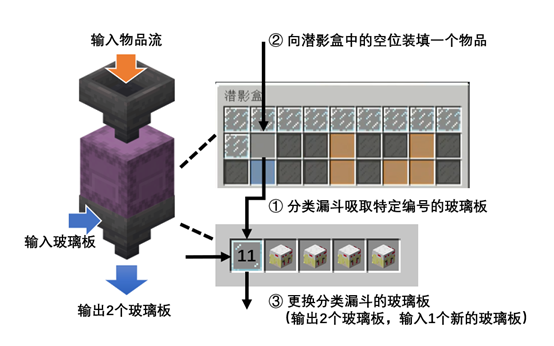
\includegraphics[width=.9\textwidth]{图片1.png}
    \label{fig:1}
    \caption{倒序装填流程图\upcite{ref1}.}
\end{figure}

根据倒序装填的原理,本文提出了一种可行的方案\upcite{ref1},流程如图\ref{fig:1}所示。预先准备一个潜影盒,每一格都填充一个玻璃板,玻璃板的命名依次为1,2,3,…,27。装填第一个物品之前,先用分类漏斗吸走27号玻璃板,再将第一个物品装入潜影盒。于是,第一个物品装进了潜影盒的第27格。装填第二个物品之前,先用分类漏斗吸走26号玻璃板,再将第二个物品装入潜影盒。由于物品优先进入靠前的格子,而潜影盒的第26格为空,那么第二个物品必定进入第26格。依次类推,每装填一个物品之前,先抽走一个玻璃板,让物品倒序地装填进潜影盒。这样,在倒序装填的过程中,虽然有相同的物品,但总有一个空的格子处在最靠前的位置,于是物品优先进入了空的格子,而不是与其他格子的物品堆叠在一起。

\begin{figure}
    \centering
    \begin{subfigure}{0.45\linewidth}
        \centering
        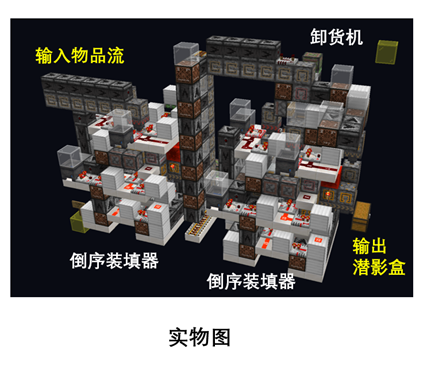
\includegraphics[width=\linewidth]{图片2.png}
        
    \end{subfigure}
    \hspace{1cm}
    \begin{subfigure}{0.45\linewidth}
        \centering
        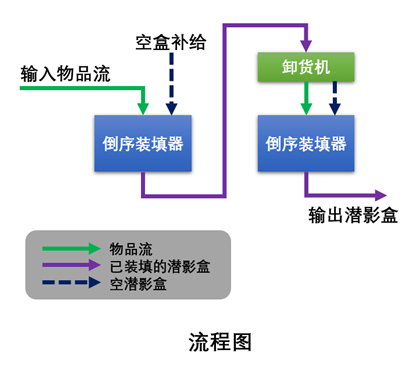
\includegraphics[width=\linewidth]{图片3.png}
        
    \end{subfigure}
    \caption{倒序装填模块}
    \label{fig:2}
\end{figure}

根据上述方案,本文设计了一种实用的倒序装填模块\upcite{ref4},如图\ref{fig:2}所示,仅需输入空潜影盒和物品流,就能输出按物品流顺序装填的潜影盒。该模块由两个倒序装填器和一个卸货机构成,两个倒序装填器串联使用,物品流经过两次倒序装填后,顺序就与原来一致了。该装置采用了一种“正序、逆序模板盒”的技术\upcite{ref5},让命名的玻璃板在机器内自循环,无需额外补充。在实际使用时\upcite{ref2,ref6},先用卸货机将潜影盒ROM中的物品逐个吸取出来,再用分类机读取物品流中的信息,最后将读取后的物品流输入倒序装填模块,最终得到与原先完全一样的潜影盒,即潜影盒ROM可重复读取。

倒序装填技术的出现,使得用可堆叠物品编码的潜影盒ROM能够重复读取。将这项技术应用到编码红石音乐领域,使得乐谱可以反复播放,让编码红石音乐机有了生存模式下的实用价值\upcite{ref6}。若将该项技术应用到红石数电领域,能作为一种高密度的存储器,提高红石计算机的存储空间,使其能容纳下更多、数据量更大的程序,具有良好的发展前景。

\bibliographystyle{unsrt}
\bibliography{reference.bib}

\end{document}

